% !TeX program = xelatex
% !TeX encoding = UTF-8
% Software Architecture Document -- adapted from the lecturer's
% simplified RUP Software Architecture Document Word template.
%
% PA4 revision: single self-contained file (metadata + layout + all sections).
% Text added or changed in PA4 is blue (\upd{...} or the updated environment).
% Build from this directory:  latexmk -xelatex main.tex

\documentclass[10pt,letterpaper]{article}
% -------------------- Metadata --------------------
% Project and document metadata only; layout belongs in main.tex.
% Project/team/organization/author names are retained from the PA2 metadata.
% Team details are carried over from the PA2 project documentation.
% Escape LaTeX special characters in values: \&, \%, \_, \#.

\newcommand{\ProjectName}{MEDICATION SAFETY ASSISTANT}
\newcommand{\GroupName}{Medication Safety Assistant Team}
\newcommand{\GroupNumber}{Group 02}
\newcommand{\OrganizationName}{University of Science, VNU-HCM}
\newcommand{\DocumentAuthors}{Cao Hoàng Long, Hoàng Yến Trang, Lỗ Chí Thành}

\newcommand{\DocumentTitle}{Software Architecture Document}
\newcommand{\DocumentPhase}{PA4}
\newcommand{\DocumentIdentifier}{PA4-Group02-SAD}
\newcommand{\DocumentVersion}{2.0}
\newcommand{\DocumentDate}{28 November 2026}
\newcommand{\DocumentYear}{2026}
\newcommand{\ConfidentialityText}{Confidential}

\newcommand{\RevisionDate}{11 Nov 2026}
\newcommand{\RevisionVersion}{1.0}
\newcommand{\RevisionDescription}{Initial PA3 Software Architecture Document template based on the instructor's simplified RUP format}
\newcommand{\RevisionAuthor}{Group 02}

% -------------------- Fonts and layout -------------------------
\usepackage{fontspec}
\defaultfontfeatures{Ligatures=TeX}
\IfFontExistsTF{Times New Roman}{%
  \setmainfont{Times New Roman}
}{%
  \IfFontExistsTF{Tinos}{%
    \setmainfont{Tinos}
  }{%
    \setmainfont{Liberation Serif}
  }%
}
\IfFontExistsTF{Arial}{\setsansfont{Arial}}{%
  \IfFontExistsTF{TeX Gyre Heros}{\setsansfont{TeX Gyre Heros}}{\setsansfont{Liberation Sans}}
}
% The instructor's RUP document uses US Letter; typography follows the PA2 Vision style.
\usepackage[letterpaper,margin=1in,headheight=34pt,headsep=16pt,
            footskip=28pt]{geometry}
\usepackage{setspace}
\setstretch{1.08}
\usepackage{microtype}
\usepackage{array,tabularx,longtable,booktabs}
\usepackage{graphicx}
\graphicspath{{images/}{figures/}}
\usepackage{float}
\usepackage{caption}
\usepackage{pdflscape}
\usepackage{enumitem}
\usepackage{titlesec}
\usepackage{fancyhdr}
\usepackage{lastpage}
\usepackage{xcolor}
\usepackage{needspace}
\usepackage{tikz}
\usetikzlibrary{positioning,shapes.geometric,arrows.meta,fit,backgrounds}
% -------- PA4 update marking: text added or changed in PA4 is blue --------
\definecolor{pafourblue}{RGB}{0,82,204}
\newcommand{\upd}[1]{{\color{pafourblue}#1}}
\newenvironment{updated}{\par\color{pafourblue}}{\par}
\usepackage{tocloft}
\usepackage[unicode,hidelinks]{hyperref}

\setlength{\parindent}{0pt}
\setlength{\parskip}{5pt}
\setlength{\tabcolsep}{5pt}
\renewcommand{\arraystretch}{1.23}
\emergencystretch=2em
\setcounter{secnumdepth}{3}
\setcounter{tocdepth}{3}
\setlist[itemize]{topsep=3pt,itemsep=2pt,parsep=0pt}
\renewcommand{\contentsname}{Table of Contents}
\titleformat{\section}{\normalfont\bfseries\fontsize{12}{15}\selectfont}{\thesection.}{0.6em}{}
\titleformat{\subsection}{\normalfont\bfseries\normalsize}{\thesubsection}{0.6em}{}
\titleformat{\subsubsection}{\normalfont\itshape\normalsize}{\thesubsubsection}{0.6em}{}
\titlespacing*{\section}{0pt}{6pt}{3pt}
\titlespacing*{\subsection}{0pt}{6pt}{3pt}
\renewcommand{\cfttoctitlefont}{\hfill\normalfont\bfseries\fontsize{17}{21}\selectfont}
\renewcommand{\cftaftertoctitle}{\hfill\mbox{}}
\setlength{\cftbeforetoctitleskip}{0pt}
\setlength{\cftaftertoctitleskip}{16pt}
\renewcommand{\cftsecfont}{\normalfont}
\renewcommand{\cftsecpagefont}{\normalfont}
\renewcommand{\cftsecaftersnum}{.}
\renewcommand{\cftsecleader}{\cftdotfill{\cftdotsep}}
\renewcommand{\cftsubsecleader}{\cftdotfill{\cftdotsep}}
\setlength{\cftbeforesecskip}{7pt}
\setlength{\cftsecnumwidth}{1.7em}
\setlength{\cftsubsecindent}{1.7em}
\setlength{\cftsubsecnumwidth}{3em}
\tocloftpagestyle{fancy}

% Compatible with section files containing figures, tables, diagrams.
\newcolumntype{L}[1]{>{\raggedright\arraybackslash}p{#1}}
\newcolumntype{Y}{>{\raggedright\arraybackslash}X}
\newcommand{\sourcefile}[1]{\nolinkurl{#1}}
\newcommand{\db}[1]{\nolinkurl{#1}}
\newcommand{\status}[1]{\textsc{#1}}
% Blue italic instructions follow the instructor's InfoBlue guidance style.
% Replace each TODO with authored content and remove the instruction wrapper.
\DeclareRobustCommand{\TODO}[1]{{\color{blue}\itshape TODO: #1}}
\newcommand{\diagramplaceholder}[4][3cm]{%
  \begin{figure}[H]
    \centering
    \fbox{\begin{minipage}[c][#1][c]{\dimexpr\linewidth-2\fboxsep-2\fboxrule\relax}
      \centering\TODO{#2}
    \end{minipage}}
    \caption{\TODO{#3}}\label{#4}
  \end{figure}%
}
\newcommand{\frontmattertitle}[1]{%
  \begin{center}{\normalfont\bfseries\fontsize{16}{20}\selectfont #1\par}\end{center}%
}
\newcommand{\portraitdiagram}[3]{%
  \begin{figure}[p]
    \centering
    \includegraphics[width=\textwidth,height=.78\textheight,
                     keepaspectratio]{#1}
    \caption{#2}\label{#3}
  \end{figure}
  \clearpage
}
\newcommand{\landscapediagram}[3]{%
  \clearpage
  \begin{landscape}
    \begin{figure}[p]
      \centering
      \includegraphics[width=\linewidth,height=.82\textheight,
                       keepaspectratio]{#1}
      \caption{#2}\label{#3}
    \end{figure}
  \end{landscape}
  \clearpage
}

% --------- Clean Vision-style running header/footer ----------
% Do not use a tabular/table here: this is a running header, not a data table.
\pagestyle{fancy}
\fancyhf{}
\fancyhead[L]{%
  \begin{minipage}[b]{.73\textwidth}
    \raggedright\fontsize{9}{11}\selectfont
    \ProjectName\\[-1pt]
    {\fontsize{8}{10}\selectfont\DocumentTitle\enspace(\DocumentIdentifier)}
  \end{minipage}%
}
\fancyhead[R]{%
  \begin{minipage}[b]{.24\textwidth}
    \raggedleft\fontsize{9}{11}\selectfont
    Version \DocumentVersion\\[-1pt]
    {\fontsize{8}{10}\selectfont\DocumentDate}
  \end{minipage}%
}
\fancyfoot[L]{\fontsize{8.5}{10}\selectfont\OrganizationName{} -- Course Project}
\fancyfoot[C]{\fontsize{8}{10}\selectfont\ConfidentialityText}
\fancyfoot[R]{\fontsize{8.5}{10}\selectfont Page \thepage\ of \pageref{LastPage}}
\renewcommand{\headrulewidth}{0.45pt}
\renewcommand{\footrulewidth}{0.45pt}
% Like the PA2 Vision cover, the title page has no running header/footer.
\fancypagestyle{sadcover}{\fancyhf{}\renewcommand{\headrulewidth}{0pt}%
  \renewcommand{\footrulewidth}{0pt}}

\hypersetup{
  pdftitle={\DocumentTitle\ - \ProjectName},
  pdfauthor={\DocumentAuthors},
  pdfsubject={\DocumentPhase\ Software Architecture}
}

\begin{document}

% ------------------ PAGE 1: Vision-style cover ------------------
\thispagestyle{sadcover}
\begin{center}
  \vspace*{.35in}
  {\bfseries\fontsize{13}{17}\selectfont \ProjectName\par}
  \vspace*{1.50in}
  {\bfseries\fontsize{22}{27}\selectfont \DocumentTitle\par}
  \vspace{8pt}
  {\fontsize{12}{16}\selectfont (Small Project)\par}
  \vspace{.92in}
  {\fontsize{12}{15}\selectfont Version \DocumentVersion\par}
  \vfill
  {\fontsize{10}{14}\selectfont
    \begin{tabular}{@{}r@{\quad}l@{}}
      \textbf{Document identifier:} & \DocumentIdentifier\\
      \textbf{Prepared by:} & \GroupNumber{} -- \GroupName\\
      \textbf{Authors:} & \DocumentAuthors\\
      \textbf{Organization:} & \OrganizationName\\
      \textbf{Date:} & \DocumentDate
    \end{tabular}\par}
  \vspace*{1.05in}
\end{center}
\clearpage

% ---------------- PAGE 2: Revision History ---------------------
\frontmattertitle{Revision History}
\vspace{7pt}
{\renewcommand{\arraystretch}{1.28}%
\begin{tabularx}{\textwidth}{|L{2.10cm}|L{1.30cm}|Y|L{2.60cm}|}
  \hline
  \textbf{Date} & \textbf{Version} & \textbf{Description} & \textbf{Author}\\
  \hline
  \RevisionDate & \RevisionVersion & \RevisionDescription & \RevisionAuthor\\
  \hline
  \upd{28 Nov 2026} & \upd{2.0} & \upd{Updated implementation status and architecture notes; completed Deployment and Implementation Views.} & \upd{Group 02}\\
  \hline
\end{tabularx}}

\medskip
\upd{\textit{Convention: text written in blue was added or changed in PA4 (version 2.0).}}
\clearpage


% ---------------- Table of Contents --------------------
\tableofcontents
\clearpage

% ---------------- List of Figures --------------------
\phantomsection
\addcontentsline{toc}{section}{List of Figures}
\listoffigures
\clearpage

% ---------------- List of Tables --------------------
\phantomsection
\addcontentsline{toc}{section}{List of Tables}
\listoftables
\clearpage

% ---------------- MAIN BODY: lecturer's exact sections ---------
\frontmattertitle{\DocumentTitle}

% 1. Overview, purpose, scope, terminology, references.
% ===== sections/01-Introduction.tex =====

\section{Introduction}
\label{sec:introduction}

\noindent\textbf{Purpose.}
This document describes the software architecture of the
\emph{Medication Safety Assistant}, including its main components,
responsibilities, interfaces, and relationships. It serves as
a technical reference for the project team and course reviewers.

\medskip
\noindent\textbf{Scope.}
The Medication Safety Assistant is a Web-based research prototype
supporting medication intake, identification, safety assessment,
simulated healthcare professional review, and medication reminders.

This document covers architectural goals and constraints,
the use-case model, and the logical view\upd{, the deployment view and
the implementation view (folder structure). Version 2.0 also records
which use cases are implemented in release v0.4.0}. The system provides
decision support only and does not replace professional medical
judgment.



\medskip
\noindent\textbf{Definitions, Acronyms and Abbreviations.}

\noindent
\begin{tabularx}{\textwidth}{|L{2.8cm}|Y|}
    \hline
    \textbf{Term} & \textbf{Definition} \\ \hline
    SAD & Software Architecture Document \\ \hline
    HCP & Healthcare Professional \\ \hline
    DDI & Drug--Drug Interaction \\ \hline
    ADR & Adverse Drug Reaction \\ \hline
    OCR & Optical Character Recognition \\ \hline
    NLP & Natural Language Processing \\ \hline
    API & Application Programming Interface \\ \hline
    DTO & Data Transfer Object \\ \hline
    RBAC & Role-Based Access Control \\ \hline
    ERD & Entity--Relationship Diagram \\ \hline
    UUID & Universally Unique Identifier \\ \hline
    Core DB V4 & \upd{The \texttt{msa} and \texttt{msa\_ref} schemas for medication,
    patient health and other business records.} \\ \hline
    Auth/RBAC & \upd{Account, authentication, role and permission tables
    in the \texttt{public} schema.} \\ \hline
    \upd{UML} & \upd{Unified Modeling Language} \\ \hline
    \upd{RLS} & \upd{Row-Level Security: PostgreSQL policies that limit
    which rows an authenticated actor can read or change.} \\ \hline
    \upd{Review case} & \upd{A patient-authorized request for an HCP to review
    a safety assessment (SAFETY) or a medication schedule (SCHEDULE).} \\ \hline
\end{tabularx}


\medskip
\noindent\textbf{References.}

\noindent
\begin{tabularx}{\textwidth}{|L{1.5cm}|Y|}
    \hline
    \textbf{ID} & \textbf{Document} \\ \hline
    R1 & Vision Document \\ \hline
    R2 & Use-Case Specification \\ \hline
    R3 & Software Development Plan \\ \hline
    \upd{R4} & \upd{PA4 Test Plan, Test Cases and Test Report} \\ \hline
    \upd{R5} & \upd{Source repository and release v0.4.0:
    \url{https://github.com/hyt2434/Medical_Safety_Assistant}} \\ \hline
\end{tabularx}

\medskip
\noindent\textbf{Overview.}
Section 2 presents architectural goals and constraints.
Section 3 presents the use-case model.
Section 4 describes the logical architecture and its components.
\upd{Section 5 presents the UML deployment diagram and describes each node.
Section 6 presents the folder structure of the source code and supporting files.}


% 2. Key non-functional requirements and constraints from Vision.
% ===== sections/02-Architectural Goals and Constraints.tex =====
% Keep Section 2 on its own page and prevent earlier floats from mixing in.
\clearpage
\section{Architectural Goals and Constraints}
\label{sec:architectural-goals}

\medskip
\noindent\textbf{Architectural Goals}

\begin{table}[!htbp]
\centering
\caption{Architectural Goals and Their Impacts}
\label{tab:architectural-goals}

\begin{tabularx}{\textwidth}{|L{3cm}|L{2cm}|Y|}
\hline
\textbf{Goal} & \textbf{Source} &
\textbf{Architectural Impact} \\ \hline

Safety and Reliability & NFR-02, NFR-03 &
Confirm medication input, handle incomplete assessments,
preserve severe warnings, and support fallback input.
\\ \hline

Security and Privacy & NFR-04 &
Enforce RBAC and patient-authorized case sharing.
\\ \hline

Data Integrity and Traceability & NFR-07, NFR-10 &
Preserve medication history, assessment results,
review decisions, and source references.
\\ \hline

Performance and Usability & NFR-01, NFR-05 &
Complete at least 90\% of standard safety checks within
10 seconds under normal conditions; provide clear
warnings and status feedback.
\\ \hline

Maintainability and Extensibility & NFR-08 &
Separate the five main modules with clearly defined
responsibilities.
\\ \hline

\upd{Testability} & \upd{PA4 Test Plan} &
\upd{Keep business rules in services and the database so they can be
tested through the REST API; run destructive integration tests only on an
isolated, marked PostgreSQL test database.}
\\ \hline

\end{tabularx}
\end{table}

\medskip
\noindent\textbf{Architectural Constraints}

\begin{table}[!htbp]
\centering
\caption{Architectural Constraints and Their Impacts}
\label{tab:architectural-constraints}

\begin{tabularx}{\textwidth}{|L{3cm}|L{2cm}|Y|}
\hline
\textbf{Constraint} & \textbf{Source} &
\textbf{Architectural Impact} \\ \hline

Web Platform & NFR-06 &
Support major desktop and mobile browsers;
provide manual input and in-app schedule viewing
when browser capabilities are unavailable.
\\ \hline

Medication Safety Rules & NFR-03, PF-07 &
Activate only verified, confirmed schedules.
Hold new reminders for medicines with severe
interactions pending HCP review; never
automatically stop existing reminders or treatment.
\\ \hline

Research Scope and Data Sources & NFR-04, NFR-10 &
Use synthetic or de-identified data and simulated HCP
review. Respect data-source permissions and
mark unsupported checks as unassessed.
\\ \hline

\upd{Database-enforced rules} & \upd{NFR-03, NFR-04} &
\upd{Consent-scoped case access, schedule verification and reminder
eligibility are enforced by PostgreSQL RLS policies and triggers
(migrations 003--005), not only by the API. Migrations are append-only:
a rule change needs a new migration file.}
\\ \hline

\end{tabularx}
\end{table}

% Finish placing both Section 2 tables before Section 3 begins.
\clearpage

% 3. Use-case diagram(s) from the Use-Case Specification document.
% ===== sections/03-Use-Case Model.tex =====

\section{Use-Case Model}
\label{sec:use-case-model}

This section presents the 20 main use cases of the
Medication Safety Assistant system. The diagrams illustrate
the interactions between actors and the system's functional
capabilities. Detailed descriptions, basic flows, alternative
flows, and conditions are provided in the
Use-Case Specification Document.

\begin{updated}
\noindent\textbf{Implementation status in release v0.4.0.}\par\smallskip
\begingroup\small
\begin{tabularx}{\textwidth}{|L{3.4cm}|Y|}
\hline
\textbf{Status} & \textbf{Use cases} \\ \hline
Implemented (server and UI) & UC-01, UC-02, UC-04, UC-05, UC-06, UC-08, UC-09, UC-11, UC-15 \\ \hline
Partially implemented & UC-03: interaction checks work, but patient-specific checks are incomplete. UC-07: reminder settings work, but timing proposals cannot carry new times. \\ \hline
UI prototype (local data) & UC-10, UC-12, UC-13, UC-14, UC-16, UC-17, UC-18, UC-20 (account viewing uses the server) \\ \hline
Future development & UC-19 \\ \hline
\end{tabularx}
\endgroup
\end{updated}


% Reusable use-case figure
\newcommand{\usecasefigure}[3]{%
    \begin{figure}[!htbp]
        \centering
        \includegraphics[
            width=0.95\linewidth,
            height=0.37\textheight,
            keepaspectratio
        ]{images/UC-#1.png}
        \caption[UC-#1: #2]{%
            \textbf{UC-#1: #2.} #3%
        }
        \label{fig:uc-#1}
    \end{figure}
}


% UC-01
\usecasefigure{01}{Sign In}{
    Allows registered users to securely access the system
    according to their assigned roles.
}

% UC-02
\usecasefigure{02}{Enter and Confirm Medication Information}{
    Allows patients to enter, review, and confirm their
    medication information before further processing.
}

% UC-03
\usecasefigure{03}{Check Medication Safety}{
    Allows patients to check potential medication risks,
    including drug interactions and other safety concerns.
}

% UC-04
\usecasefigure{04}{Arrange HCP Review}{
    Supports authorized HCP review requests, case
    assignment, and review status tracking.
}

% UC-05
\usecasefigure{05}{Review Medication Safety Case}{
    Allows healthcare professionals to review authorized
    safety cases and communicate with patients.
}

% UC-06
\usecasefigure{06}{Set Up Medication Reminders}{
    Allows patients to set up and confirm medication reminders
    based on verified schedules, with HCP review when required.
}

% UC-07
\usecasefigure{07}{Manage Medication Reminders}{
    Allows patients to adjust notification settings and
    propose medication timing changes subject to HCP review.
}

% UC-08
\usecasefigure{08}{Record Dose Status}{
    Allows patients to record and confirm their
    medication-taking status.
}

% UC-09
\usecasefigure{09}{View Adherence History}{
    Allows patients to view, filter, and summarize
    their medication adherence history.
}

% UC-10
\usecasefigure{10}{View Medication and Safety History}{
    Allows patients to view medication records, examine past
    safety assessments, and compare assessment results.
}

% UC-11
\usecasefigure{11}{Ask a Medication Question}{
    Allows patients to ask medication-related questions,
    view chatbot conversation history, and access supporting references.
}

% UC-12
\usecasefigure{12}{Generate Patient Health Summary}{
    Allows patients to generate, review, and confirm
    a structured summary of their health information.
}

% UC-13
\usecasefigure{13}{Share Patient Health Summary with HCP}{
    Allows patients to share health summaries with authorized HCPs,
    confirm sharing permissions, and revoke access when needed.
}

% UC-14
\usecasefigure{14}{Review Medication Reference Data}{
    Allows dataset reviewers to verify reference data against
    supporting evidence, record quality decisions, and review history.
}

% UC-15
\usecasefigure{15}{Manage User Accounts and Roles}{
    Allows administrators to create and deactivate accounts,
    assign roles, reset passwords, and view account activity history.
}

% UC-16
\usecasefigure{16}{Report Technical Issue}{
    Allows registered users to report technical issues,
    review attachments, reply to support tickets,
    and track ticket status.
}

% UC-17
\usecasefigure{17}{Handle Technical Support Request}{
    Allows technical support staff to view assigned tickets,
    investigate issues, request additional information,
    and manage ticket resolution.
}

% UC-18
\usecasefigure{18}{Manage Patient Health Profile}{
    Allows patients to manage medical conditions, allergies,
    medication and adverse reaction histories,
    lifestyle information, and health measurements.
}

% UC-19
\usecasefigure{19}{Manage Personal Medication Cabinet}{
    Allows patients to add and update personal medicines,
    track usage status, view medication details and known
    side effects, and monitor expiration dates.
}

% UC-20
\usecasefigure{20}{Manage Personal Account}{
    Allows registered users to view and update their
    personal account information and change passwords.
}

\clearpage


% 4. Architecture diagrams; component responsibilities, services,
%    communications (HTTP/HTTPS/etc.); class diagrams for components.
%    Add \subsection{Component: <name>} for each component.
% ===== sections/04-Logical View.tex =====
% ============================================================
% SECTION 4 - LOGICAL VIEW (INTRODUCTION + COMPONENT OVERVIEW)
% Medication Safety Assistant - PA3
%
% Paste this section before Component 4.1 (Web Frontend).
% Requires: graphicx, caption, fancyhdr, tabularx.
% Table column types L{...} and Y must be defined in main.tex.
% Compile with XeLaTeX to use upright landscape pages.
% Image: images/Component_Overview.png
% The existing numbered component diagrams use images/01.png ...
% and the \LogicalComponentPage macro below.
% ============================================================

\section{Logical View}
\label{sec:logical-view}

The Medication Safety Assistant uses a \textbf{three-tier layered modular monolith}.
The frontend shows the user interface and the Python backend runs the business logic.
\upd{In the unified PostgreSQL deployment, \texttt{msa} and \texttt{msa\_ref}
hold business data, \texttt{public} holds Auth/RBAC data, and \texttt{identity}
links user identifiers.} The twelve components are logical parts of one system, not separate
microservices.

\noindent\textbf{Architecture and communication.}\par\smallskip
\begingroup\small
\begin{tabularx}{\textwidth}{|L{0.24\textwidth}|Y|}
\hline
\textbf{Tier} & \textbf{Technology and responsibility} \\ \hline
Presentation & TypeScript, HTML and CSS; display pages and collect user input. \\ \hline
Application & Python API and services; validate requests, check permissions and run business logic. \\ \hline
Data & \upd{Python repositories and logically separated PostgreSQL schemas; save records and audit events.} \\ \hline
\end{tabularx}
\endgroup

The frontend communicates with the API using \textbf{HTTPS/JSON} (HTTP may be
used locally). Backend services communicate through \textbf{Python calls}
and typed data objects. Repositories use \textbf{parameterized SQL} and
transactions to access Core DB V4.

\noindent\textbf{Component overview.}\par\smallskip
\begingroup\small\renewcommand{\arraystretch}{1.08}
\begin{tabularx}{\textwidth}{|L{0.43\textwidth}|Y|}
\hline
\textbf{Component} & \textbf{Main responsibility} \\ \hline
Web Frontend & Show role-based pages and send user actions. \\ \hline
API Controllers & Validate, authorize and route requests. \\ \hline
Medication Intake and Chatbot (M1) & Collect, clarify and confirm medication information. \\ \hline
Medication Identification (M2) & Find medication candidates and identify ingredients. \\ \hline
Safety Assessment and Decision Support (M3) & Check supported risks and record safety findings. \\ \hline
HCP Review and Patient Health Summary (M4) & Manage permitted reviews and patient-approved summaries. \\ \hline
Reminders and Adherence (M5) & Manage eligible reminders and dose history. \\ \hline
Patient Health Profile & Keep reported health information and medication-use status. \\ \hline
Reference Data and Dataset Review & Provide versioned drug data and store review decisions. \\ \hline
Account and Access Management & Manage accounts, sessions, roles and access rules. \\ \hline
Technical Support & Handle technical support tickets and messages. \\ \hline
Data Persistence and Audit & Provide database access, transactions and audit records. \\ \hline
\end{tabularx}
\endgroup

\noindent\textbf{Main component communication.}\par\smallskip
\begingroup\small\renewcommand{\arraystretch}{1.08}
\begin{tabularx}{\textwidth}{|L{0.34\textwidth}|L{0.23\textwidth}|Y|}
\hline
\textbf{Connection} & \textbf{Means} & \textbf{Purpose} \\ \hline
Frontend to API & HTTPS/JSON & Send user requests and return results. \\ \hline
API to backend services & Python calls & Route validated and authorized requests. \\ \hline
M1 to M2 to M3 & Typed data objects & Pass confirmed entries and identification results. \\ \hline
M3 and M4 to M5 & Gate and review results & Check reminder eligibility before activation. \\ \hline
M2/M3 to Reference Data & Python calls & Read drug, ingredient and DDI references. \\ \hline
M3/M4 to Health Profile & Python calls & Read permitted health context and summary data. \\ \hline
Services to Persistence & Repository calls & Read and save permitted records. \\ \hline
Persistence to PostgreSQL & SQL/transactions & Access Core DB V4. \\ \hline
\end{tabularx}
\endgroup

\noindent\textbf{Safety and access rules.}\par\smallskip
Patient confirmation does not prove medication identity or clinical safety.
Unknown medicines and unsupported checks remain \emph{Unassessed}.
Severe drug interactions can hold new reminders for affected medicines;
treatment and existing reminders are not changed automatically.
An HCP review requires authorized case access. Sharing a health summary
requires separate patient permission. UC-19 is planned for the future.

% ------------------------------------------------------------
% Page helpers: true landscape paper, no rotated PDF content.
% These are also used by Components 4.1--4.12 below.
% ------------------------------------------------------------
\makeatletter
\providecommand{\LogicalResetPageColumns}{%
  \global\@colht\textheight
  \global\@colroom\textheight
  \global\vsize\textheight
}
\makeatother

% Arguments: {component heading}{subsection label}{introduction}
%            {PNG number}{figure label}
\newcommand{\LogicalComponentPage}[5]{%
  \par\clearpage
  \begingroup
  \setlength{\paperwidth}{297mm}%
  \setlength{\paperheight}{210mm}%
  \special{papersize=297mm,210mm}%
  \setlength{\textwidth}{261mm}%
  \setlength{\columnwidth}{\textwidth}%
  \setlength{\linewidth}{\textwidth}%
  \setlength{\hsize}{\textwidth}%
  \setlength{\headwidth}{\textwidth}%
  \setlength{\textheight}{153mm}%
  \LogicalResetPageColumns
  \setlength{\oddsidemargin}{-7.4mm}%
  \setlength{\evensidemargin}{-7.4mm}%
  \thispagestyle{fancy}%
  \subsection{#1}\label{#2}%
  \vspace{-1mm}%
  {\small #3\par}%
  \vspace{2mm}%
  \begin{center}
    \IfFileExists{images/#4.png}{%
      \includegraphics[width=0.98\textwidth,height=0.70\textheight,keepaspectratio]{images/#4.png}%
    }{%
      \fbox{\parbox[c][0.48\textheight][c]{0.80\textwidth}{\centering Missing class diagram: images/#4.png}}%
    }%
    \par\smallskip
    \captionof{figure}{#1 -- UML class diagram.}\label{#5}%
  \end{center}
  \par\clearpage
  \endgroup
  \LogicalResetPageColumns
  \special{papersize=\the\paperwidth,\the\paperheight}%
}

% ------------------------------------------------------------
% OVERALL COMPONENT DIAGRAM
% One fixed landscape page: introduction, image and caption together.
% No figure float; no extra caption-only page.
% Keep this block before Component 4.1.
% Image: images/Component_Overview.png
% ------------------------------------------------------------
\clearpage
\begingroup
  % Use a true landscape PDF page (no rotation in the PDF viewer).
  \setlength{\paperwidth}{297mm}%
  \setlength{\paperheight}{210mm}%
  \special{papersize=297mm,210mm}%
  \setlength{\textwidth}{261mm}%
  \setlength{\columnwidth}{\textwidth}%
  \setlength{\linewidth}{\textwidth}%
  \setlength{\hsize}{\textwidth}%
  \setlength{\headwidth}{\textwidth}%
  \setlength{\textheight}{153mm}%
  \LogicalResetPageColumns
  \setlength{\oddsidemargin}{-7.4mm}%
  \setlength{\evensidemargin}{-7.4mm}%
  \thispagestyle{fancy}%

  % A single, non-breaking block prevents a caption-only page.
  \noindent\begin{minipage}[t]{\textwidth}
    \textbf{Overall Component Diagram}\par\smallskip
    {\small
      Figure~\ref{fig:logical-component-overview} shows the twelve components
      in three tiers and their main connections. The frontend uses HTTPS/JSON,
      backend services use Python calls, and repositories use SQL transactions.\par
    }
    \vspace{2mm}%
    \centering
    \IfFileExists{images/Component_Overview.png}{%
      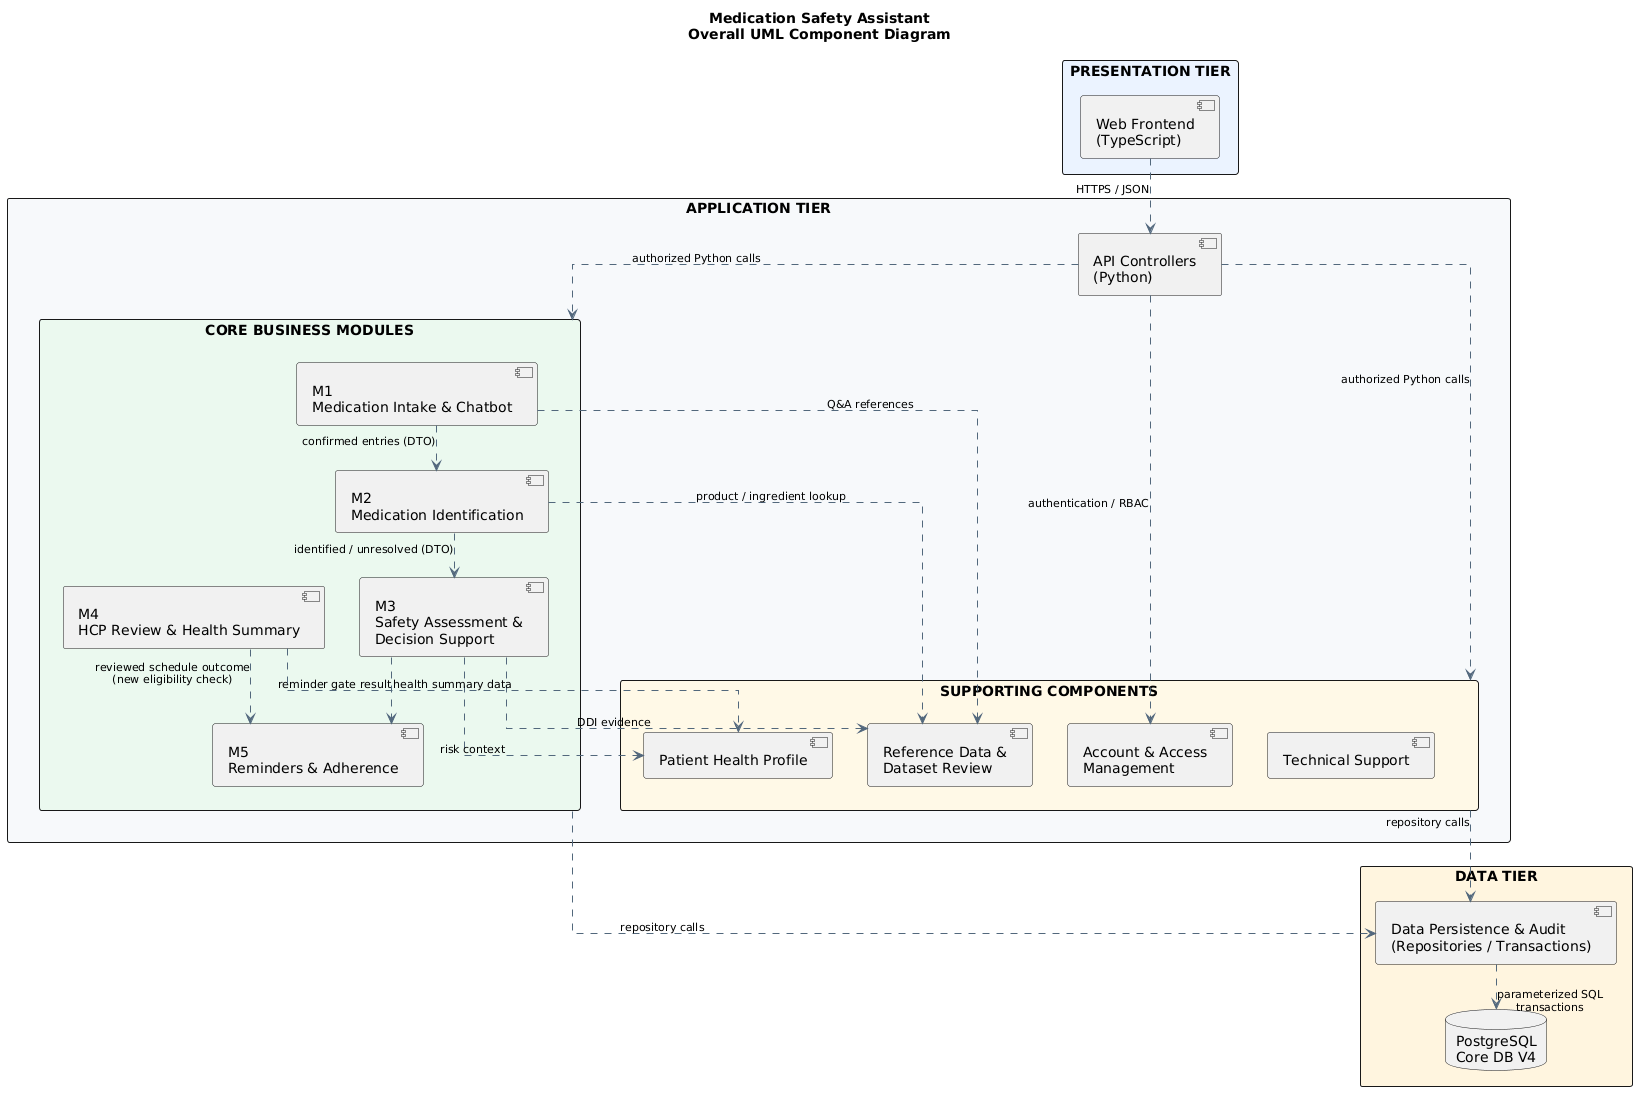
\includegraphics[
        width=0.97\linewidth,
        height=0.82\textheight,
        keepaspectratio
      ]{images/Component_Overview.png}%
    }{%
      \fbox{\parbox[c][62mm][c]{0.8\linewidth}{%
        \centering Missing diagram: images/Component\_Overview.png}}%
    }%
    \par\vspace{1mm}%
    \captionof{figure}{Medication Safety Assistant -- Overall UML component diagram.}%
    \label{fig:logical-component-overview}%
  \end{minipage}%
  \par\clearpage
\endgroup
\LogicalResetPageColumns

% ============================================================
% 4.1 - WEB FRONTEND
% ============================================================
\LogicalComponentPage{Component: Web Frontend}{subsec:logical-frontend}{%
\textbf{Purpose.} Show role-based screens, collect user actions and display
results from the backend. The frontend does not decide whether a medicine is safe.
\textbf{Related use cases:} UC-01--UC-18 and UC-20 (role-dependent).
}{01}{fig:logical-frontend-classes}

\noindent\textbf{Main classes and operations.}\par\smallskip
\begingroup\small
\begin{tabularx}{\textwidth}{|L{0.37\textwidth}|Y|}
\hline
\textbf{Class} & \textbf{Role and main operations} \\ \hline
\texttt{WebAppShell} & Coordinate role-based pages and feedback; \texttt{navigateTo()}, \texttt{showWorkflowResult()}, \texttt{showFeedback()}. \\ \hline
\texttt{ApiClient} & Provide shared API access for the views; \texttt{submitAction()}, \texttt{fetchViewData()}. \\ \hline
\texttt{MedicationEntryView} & Submit and confirm medication entries; \texttt{submitEntry()}, \texttt{confirmEntry()}. \\ \hline
\texttt{SafetyResultsView} & Show warnings and allow a user to request review; \texttt{loadSafetyReport()}, \texttt{requestHCPReview()}. \\ \hline
\texttt{ReminderView} & Display reminders and record dose status; \texttt{updateReminder()}, \texttt{recordDoseStatus()}. \\ \hline
\texttt{HCPReviewView} & View permitted cases, send messages and submit review outcomes. \\ \hline
\end{tabularx}
\endgroup

\noindent\textbf{Key relationships and their purposes.}\par\smallskip
\texttt{WebAppShell} depends on the four View classes (Dependency) to
show the screen for each user task. Each View has an Association with
\texttt{ApiClient} to send requests and display results without handling
HTTP calls itself. \texttt{ApiClient} calls API Controllers using HTTPS/JSON.


% ============================================================
% 4.2 - API CONTROLLERS
% ============================================================
\LogicalComponentPage{Component: API Controllers}{subsec:logical-api}{%
\textbf{Purpose.} Receive user requests, check their input and access rights,
then send valid requests to the right backend service.
\textbf{Related use cases:} All active use cases using the API.
}{02}{fig:logical-api-classes}

\noindent\textbf{Main classes and operations.}\par\smallskip
\begingroup\small
\begin{tabularx}{\textwidth}{|L{0.37\textwidth}|Y|}
\hline
\textbf{Class} & \textbf{Role and main operations} \\ \hline
\texttt{ApiController} & Handle HTTP requests and route commands; \texttt{handleRequest()}, \texttt{dispatch()}. \\ \hline
\texttt{RequestValidator} & Check request fields before service calls; \texttt{validate()}, \texttt{parseCommand()}. \\ \hline
\texttt{AccessGuard} & Check roles and resource permissions; \texttt{authorizeRequest()}. \\ \hline
\texttt{RequestContext} & Provide trusted user and request details for access checks; \texttt{isAuthenticated()}. \\ \hline
\end{tabularx}
\endgroup

\noindent\textbf{Key relationships and their purposes.}\par\smallskip
\texttt{ApiController} has Associations with \texttt{RequestValidator}
and \texttt{AccessGuard} so every request can be checked before routing.
Both \texttt{ApiController} and \texttt{AccessGuard} depend on
\texttt{RequestContext} for the authenticated user and request details.

\noindent\textbf{Important rule.} User identity and roles come from server-side
authentication, not from fields submitted by the user.


% ============================================================
% 4.3 - MEDICATION INTAKE AND CHATBOT (MODULE 1)
% ============================================================
\LogicalComponentPage{Component: Medication Intake and Chatbot (Module 1)}{subsec:logical-intake}{%
\textbf{Purpose.} Collect medication details from manual, OCR, chat and voice
input. Clarify missing details, prepare drafts and confirm entries before
identification. Answer supported medication questions.
\textbf{Related use cases:} UC-02 and UC-11.
}{03}{fig:logical-intake-classes}

\noindent\textbf{Main classes and operations.}\par\smallskip
\begingroup\small
\begin{tabularx}{\textwidth}{|L{0.37\textwidth}|Y|}
\hline
\textbf{Class} & \textbf{Role and main operations} \\ \hline
\texttt{ManualInputAdapter} & Prepare medication drafts from form data; \texttt{parseForm()}. \\ \hline
\texttt{OCRInputAdapter} & Prepare draft medicine data from images; \texttt{extractEntries()}. \\ \hline
\texttt{ChatInputAdapter} & Detect intent and extract draft entries from text; \texttt{detectIntent()}, \texttt{extractEntries()}. \\ \hline
\texttt{VoiceInputAdapter} & Transcribe audio and pass text to Chat; \texttt{transcribe()}, \texttt{processVoice()}. \\ \hline
\texttt{IntakeService} & Start, clarify, confirm and cancel workflows; \texttt{startIntake()}, \texttt{clarifyEntry()}, \texttt{confirmEntry()}, \texttt{cancelWorkflow()}, \texttt{buildHandoffDTO()}. \\ \hline
\texttt{IntakeValidator} & Check missing fields and uncertainty; \texttt{validate()}, \texttt{findMissingFields()}, \texttt{hasUncertainty()}. \\ \hline
\texttt{MedicationQAService} & Handle medication questions separately from intake; \texttt{answerQuestion()}. \\ \hline
\texttt{MedicationEntry} & Store raw medication fields, source and status; \texttt{updateDraft()}, \texttt{isConfirmed()}. \\ \hline
\end{tabularx}
\endgroup

\noindent\textbf{Key relationships and their purposes.}\par\smallskip
\texttt{IntakeService} depends on the four input adapters to support
different input methods. \texttt{VoiceInputAdapter} depends on
\texttt{ChatInputAdapter} to process transcribed speech as text.
\texttt{IntakeService} has Associations with \texttt{IntakeValidator}
for clarification and \texttt{MedicationQAService} for questions.
The input adapters, service and validator depend on \texttt{MedicationEntry}
to work with the same draft information.

\noindent\textbf{Important rule.} Every medication draft needs explicit user
confirmation; confirmation does not prove its identity or safety.


% ============================================================
% 4.4 - MEDICATION IDENTIFICATION (MODULE 2)
% ============================================================
\LogicalComponentPage{Component: Medication Identification (Module 2)}{subsec:logical-identification}{%
\textbf{Purpose.} Match confirmed medication entries with reviewed products
and find their ingredients. Keep unknown or unclear matches unresolved.
\textbf{Related use cases:} UC-02 and UC-03.
}{04}{fig:logical-identification-classes}

\noindent\textbf{Main classes and operations.}\par\smallskip
\begingroup\small
\begin{tabularx}{\textwidth}{|L{0.37\textwidth}|Y|}
\hline
\textbf{Class} & \textbf{Role and main operations} \\ \hline
\texttt{MedicationIdentificationService} & Coordinate matching, user selection and ingredient lookup; \texttt{identifyConfirmedEntry()}, \texttt{confirmCandidate()}, \texttt{resolveIngredients()}. \\ \hline
\texttt{MedicationMatcher} & Find products that match an entry; \texttt{findCandidates()}. \\ \hline
\texttt{IngredientResolver} & Get linked active ingredients; \texttt{resolveIngredients()}. \\ \hline
\texttt{MedicationCandidate} & Represent each possible product with confidence and source details. \\ \hline
\texttt{IdentificationResult} & Group candidate products and the selected result; \texttt{isResolved()}, \texttt{needsConfirmation()}. \\ \hline
\end{tabularx}
\endgroup

\noindent\textbf{Key relationships and their purposes.}\par\smallskip
\texttt{MedicationIdentificationService} has Associations with
\texttt{MedicationMatcher} to find products and \texttt{IngredientResolver}
to obtain their ingredients. It depends on \texttt{IdentificationResult}
to return the outcome; \texttt{MedicationMatcher} depends on
\texttt{MedicationCandidate} to create suggestions. An
\texttt{IdentificationResult} owns zero or more candidates
(Composition, 1 to 0..*) so each result groups its own suggestions.

\noindent\textbf{Important rule.} A possible match is not a confirmed identity
or a clinical safety decision.


% ============================================================
% 4.5 - SAFETY ASSESSMENT AND DECISION SUPPORT (MODULE 3)
% ============================================================
\LogicalComponentPage{Component: Safety Assessment and Decision Support (Module 3)}{subsec:logical-safety}{%
\textbf{Purpose.} Check supported medication risks and return findings with
evidence or an unassessed status. Severe or unresolved risks start a pending
HCP review request; patient permission is needed before case sharing.
\textbf{Related use cases:} UC-03, UC-06 and UC-10.
}{05}{fig:logical-safety-classes}

\noindent\textbf{Main classes and operations.}\par\smallskip
\begingroup\small
\begin{tabularx}{\textwidth}{|L{0.37\textwidth}|Y|}
\hline
\textbf{Class} & \textbf{Role and main operations} \\ \hline

\texttt{SafetyAssessmentService} &
Coordinate checks, save results and flag review needs;
\texttt{assessSafety()}, \texttt{requiresHCPReview()},
\texttt{evaluateReminderGate()}, \texttt{getReport()}. \\ \hline

\texttt{InteractionChecker} &
Check DDI severity and duplicate ingredients;
\texttt{checkInteractions()},
\texttt{checkDuplicateIngredients()}. \\ \hline

\texttt{PatientRiskChecker} &
Check patient-specific risks using available health data. \\ \hline

\texttt{SafetyGate} &
Assess new-reminder eligibility using a report and verified
schedule; \texttt{evaluate()}. \\ \hline

\texttt{SafetyReport} &
Keep evidence, missing checks and results for later review; \texttt{hasSevereDDI()},
\texttt{hasUnassessedItems()}. \\ \hline

\end{tabularx}
\endgroup

\noindent\textbf{Key relationships and their purposes.}\par\smallskip
\texttt{SafetyAssessmentService} has Associations with
\texttt{InteractionChecker} and \texttt{PatientRiskChecker} to run
different risk checks. It also uses \texttt{SafetyGate} to assess new
reminder eligibility. The service depends on \texttt{SafetyReport} to
return findings; \texttt{SafetyGate} depends on that report to use the
same results instead of repeating risk checks.

\noindent\textbf{Important rules.} Severe or unresolved findings create a request
with status \texttt{PENDING\_CONSENT}. M4 may share and assign the case only
after patient permission. Unsupported checks remain \emph{Unassessed}.
The safety gate can hold affected new reminders, never treatment.


% ============================================================
% 4.6 - HCP REVIEW AND PATIENT HEALTH SUMMARY (MODULE 4)
% ============================================================
\LogicalComponentPage{Component: HCP Review and Patient Health Summary (Module 4)}{subsec:logical-review}{%
\textbf{Purpose.} Manage permitted simulated HCP reviews and patient health
summaries. Keep case access separate from summary-sharing permission.
\textbf{Related use cases:} UC-04, UC-05, UC-12 and UC-13.
}{06}{fig:logical-review-classes}

\noindent\textbf{Main classes and operations.}\par\smallskip
\begingroup\small
\noindent\begin{tabularx}{\textwidth}{|L{0.37\textwidth}|Y|}
\hline
\textbf{Class} & \textbf{Role and main operations} \\ \hline
\texttt{ReviewCaseService} & Open cases, assign reviewers, add messages and save outcomes; \texttt{openReviewCase()}, \texttt{assignReviewer()}, \texttt{addCaseMessage()}, \texttt{recordReviewOutcome()}. \\ \hline
\texttt{ReviewConversation} & Keep the messages exchanged in a review case; \texttt{addMessage()}, \texttt{getMessages()}. \\ \hline
\texttt{ReviewOutcome} & Store each review outcome for later checking; \texttt{isScheduleVerified()}. \\ \hline
\texttt{HealthSummaryService} & Generate, confirm, share and revoke health summaries; \texttt{generateHealthSummary()}, \texttt{confirmSummary()}, \texttt{shareConfirmedSummary()}, \texttt{revokeSummarySharing()}. \\ \hline
\texttt{SharingPermissionService} & Apply separate permission checks for cases and summaries; \texttt{grantCaseAccess()}, \texttt{canAccessCase()}, \texttt{grantSummarySharing()}, \texttt{revokeSummarySharing()}, \texttt{canViewSummary()}. \\ \hline
\end{tabularx}\par
\endgroup

\noindent\textbf{Key relationships and their purposes.}\par\smallskip
\texttt{ReviewCaseService} has an Association with
\texttt{SharingPermissionService} to check permission before HCP case
access. \texttt{HealthSummaryService} has a separate Association with
the same permission service because summary sharing needs its own consent.
\texttt{ReviewCaseService} depends on \texttt{ReviewConversation} to
manage messages and on \texttt{ReviewOutcome} to record decisions.

\noindent\textbf{Important rules.} HCP case access and health-summary sharing
need separate patient permissions. Review outcomes do not change treatment
automatically.

\begin{updated}
\noindent\textbf{Implementation in release v0.4.0.} \texttt{HcpService}
handles consent-based case access, messages and review outcomes. Database
permissions restrict case access. Health-summary generation and sharing
(UC-12, UC-13) remain UI prototypes; case consent does not grant summary access.
\end{updated}


% ============================================================
% 4.7 - REMINDERS AND ADHERENCE (MODULE 5)
% ============================================================
\LogicalComponentPage{Component: Reminders and Adherence (Module 5)}{subsec:logical-reminders}{%
\textbf{Purpose.} Manage reminders based on verified medication schedules
and safety eligibility. Record dose status and requests to change timing.
\textbf{Related use cases:} UC-06--UC-09.
}{07}{fig:logical-reminders-classes}

\noindent\textbf{Main classes and operations.}\par\smallskip
\begingroup\small
\noindent\begin{tabularx}{\textwidth}{|L{0.37\textwidth}|Y|}
\hline
\textbf{Class} & \textbf{Role and main operations} \\ \hline
\texttt{ReminderService} & Set up reminders, change notification settings, submit timing proposals and manage dose records; \texttt{setupReminder()}, \texttt{updateNotificationSettings()}, \texttt{proposeScheduleChange()}, \texttt{recordDoseStatus()}, \texttt{getAdherenceHistory()}. \\ \hline
\texttt{ReminderEligibilityGate} & Check a verified schedule and the Module 3 gate result; \texttt{evaluate()}. \\ \hline
\texttt{ScheduleChangeRequest} & Keep a proposed time, request status and date without applying the change; \texttt{isPending()}. \\ \hline
\texttt{DoseStatusService} & Record confirmed \texttt{TAKEN}, \texttt{MISSED} or \texttt{SKIPPED} status; \texttt{recordDoseStatus()}. \\ \hline
\texttt{AdherenceHistoryService} & Retrieve permitted dose history for adherence views; \texttt{getHistory()}. \\ \hline
\end{tabularx}\par
\endgroup

\noindent\textbf{Key relationships and their purposes.}\par\smallskip
\texttt{ReminderService} has Associations with
\texttt{ReminderEligibilityGate} to check whether a reminder can be
activated, \texttt{DoseStatusService} to record doses, and
\texttt{AdherenceHistoryService} to show dose history. It depends on
\texttt{ScheduleChangeRequest} to store proposed timing changes without
applying them immediately.

\noindent\textbf{Important rules.} New reminders need a verified schedule and
a valid safety result. Proposed timing changes need HCP review; treatment
and existing reminders are not changed automatically.

\begin{updated}
\noindent\textbf{Implementation in release v0.4.0.} \texttt{ReminderService}
manages schedules, reminder settings, dose records and adherence history.
New reminders need a valid safety result and HCP review when required.
Notifications are in-app only. Timing proposals cannot yet carry new times;
see defects B005/B006 in the Test Report.
\end{updated}


% ============================================================
% 4.8 - PATIENT HEALTH PROFILE
% ============================================================
\LogicalComponentPage{Component: Patient Health Profile}{subsec:logical-profile}{%
\textbf{Purpose.} Keep patient-reported health facts, allergies, conditions,
previous adverse drug reactions, lifestyle details and medication-use history.
Keep their sources so M3 and M4 can use the available health context.
\textbf{Related use cases:} UC-18; supports UC-03 and UC-12.
}{08}{fig:logical-profile-classes}

\noindent\textbf{Main classes and operations.}\par\smallskip
\begingroup\small
\noindent\begin{tabularx}{\textwidth}{|L{0.37\textwidth}|Y|}
\hline
\textbf{Class} & \textbf{Role and main operations} \\ \hline
\texttt{PatientProfileService} & Save and read health and medication-use entries; \texttt{updateHealthEntry()}, \texttt{updateMedicationUse()}, \texttt{getHealthEntries()}, \texttt{getMedicationHistory()}, \texttt{getRiskContext()}. \\ \hline
\texttt{ProfileValidator} & Check reported health and medicine-use details; \texttt{validateHealthEntry()}, \texttt{validateMedicationUse()}. \\ \hline
\texttt{HealthProfileEntry} & Keep entry type, raw value, source, reported time and patient confirmation; \texttt{isConfirmed()}. \\ \hline
\texttt{MedicationUseEntry} & Keep medicine name, current/discontinued status, dates, source and patient confirmation; \texttt{isCurrentlyUsed()}, \texttt{isConfirmed()}. \\ \hline
\end{tabularx}\par
\endgroup

\noindent\textbf{Key relationships and their purposes.}\par\smallskip
\texttt{PatientProfileService} has an Association with
\texttt{ProfileValidator} to check reported information before saving it.
It depends on \texttt{HealthProfileEntry} and \texttt{MedicationUseEntry}
to keep health facts and medicine-use records separately.
\texttt{ProfileValidator} also depends on these two entry classes to
check the fields relevant to each type.

\noindent\textbf{Important rule.} Patient confirmation is not clinical
verification. Current and discontinued medicines remain separate.


% ============================================================
% 4.9 - REFERENCE DATA AND DATASET REVIEW
% ============================================================
\LogicalComponentPage{Component: Reference Data and Dataset Review}{subsec:logical-reference}{%
\textbf{Purpose.} Provide reviewed, versioned medicine and ingredient data
for identification and safety checks. Let Dataset Reviewers record decisions
with supporting evidence.
\textbf{Related use cases:} UC-14; supports UC-02, UC-03 and UC-11.
}{09}{fig:logical-reference-classes}

\noindent\textbf{Main classes and operations.}\par\smallskip
\begingroup\small
\noindent\begin{tabularx}{\textwidth}{|L{0.34\textwidth}|Y|}
\hline
\textbf{Class} & \textbf{Role and main operations} \\ \hline
\texttt{DatasetReviewService} & Open records, propose corrections and save review decisions; \texttt{openRecord()}, \texttt{proposeCorrection()}, \texttt{decide()}. \\ \hline
\texttt{ReferenceCatalog} & Find products, read source and DDI evidence, and keep review history; \texttt{findCandidates()}, \texttt{getRecord()}, \texttt{getInteractionEvidence()}, \texttt{appendDecision()}. \\ \hline
\texttt{ReviewDecision} & Keep who reviewed which record, the decision and its evidence; \texttt{isAccepted()}, \texttt{getRationale()}. \\ \hline
\end{tabularx}\par
\endgroup

\noindent\textbf{Key relationships and their purposes.}\par\smallskip
\texttt{DatasetReviewService} has an Association with
\texttt{ReferenceCatalog} to open source-linked records and check their
evidence. It depends on \texttt{ReviewDecision} to record the review result.
\texttt{ReferenceCatalog} has an Association (1 to 0..*) with
\texttt{ReviewDecision} so one catalog can keep many review decisions.

\noindent\textbf{Important rule.} A dataset review decision does not directly
change released reference records or prove clinical safety.


% ============================================================
% 4.10 - ACCOUNT AND ACCESS MANAGEMENT
% ============================================================
\LogicalComponentPage{Component: Account and Access Management}{subsec:logical-accounts}{%
\textbf{Purpose.} Manage accounts, login sessions, passwords and roles.
Check access rights before protected actions and prevent unauthorized
account changes.
\textbf{Related use cases:} UC-01, UC-15 and UC-20.
}{10}{fig:logical-accounts-classes}

\noindent\textbf{Main classes and operations.}\par\smallskip
\begingroup\small
\noindent\begin{tabularx}{\textwidth}{|L{0.34\textwidth}|Y|}
\hline
\textbf{Class} & \textbf{Role and main operations} \\ \hline

\texttt{AccountService} &
Manage sign-in, accounts, passwords and roles;
\texttt{login()}, \texttt{logout()}, \texttt{switchContext()},
\texttt{createAccount()}, \texttt{deactivateAccount()},
\texttt{resetPassword()}, \texttt{updatePersonalDetails()},
\texttt{changePassword()}, \texttt{grantRole()},
\texttt{revokeRole()}. \\ \hline

\texttt{RBACPolicy} &
Check permissions, account ownership and admin-role rules;
\texttt{hasPermission()}, \texttt{requireOwner()},
\texttt{canRevokeAdmin()}. \\ \hline

\texttt{UserAccount} &
Keep account details and assigned roles;
\texttt{verifyPassword()}, \texttt{isActive()},
\texttt{getActiveRoles()}, \texttt{addGrant()},
\texttt{revokeGrant()}. \\ \hline

\texttt{AuthSession} &
Keep login sessions and the selected role;
\texttt{isValid()}, \texttt{selectContext()},
\texttt{rotateToken()}, \texttt{invalidate()}. \\ \hline

\texttt{Role} &
Define permissions shared by users with a role;
\texttt{hasPermission()}. \\ \hline

\texttt{RoleGrant} &
Keep the history and validity of each role assignment;
\texttt{isActive()}, \texttt{revoke()}. \\ \hline

\end{tabularx}\par
\endgroup

\noindent\textbf{Key relationships and their purposes.}\par\smallskip
\texttt{AccountService} has an Association with \texttt{RBACPolicy}
to check allowed account actions and depends on \texttt{UserAccount} and
\texttt{AuthSession} to manage users and sign-in. \texttt{RBACPolicy}
depends on \texttt{AuthSession} to check the selected role.
\texttt{AuthSession} is associated with \texttt{UserAccount} and
\texttt{Role}. \texttt{UserAccount} owns its \texttt{RoleGrant}
records (Composition, 1 to 0..*); each \texttt{RoleGrant} is associated
with a \texttt{Role} to identify the granted permissions.

\noindent\textbf{Important rule.} A role alone does not grant access to patient
health data. Ownership and case-specific permission must also be checked.


% ============================================================
% 4.11 - TECHNICAL SUPPORT
% ============================================================
\LogicalComponentPage{Component: Technical Support}{subsec:logical-support}{%
\textbf{Purpose.} Let users report technical problems and track requests.
Let authorized support staff handle assigned tickets and replies.
\textbf{Related use cases:} UC-16 and UC-17.
}{11}{fig:logical-support-classes}

\noindent\textbf{Main classes and operations.}\par\smallskip
\begingroup\small
\noindent\begin{tabularx}{\textwidth}{|L{0.34\textwidth}|Y|}
\hline
\textbf{Class} & \textbf{Role and main operations} \\ \hline
\texttt{SupportTicketService} & Create, assign and update tickets, and add replies; \texttt{createTicket()}, \texttt{listAssignedTickets()}, \texttt{assignTicket()}, \texttt{addReply()}, \texttt{updateTicketStatus()}. \\ \hline
\texttt{TicketAccessPolicy} & Check permission to view, reply to or update a ticket; \texttt{canView()}, \texttt{canReply()}, \texttt{canUpdateStatus()}. \\ \hline
\texttt{SupportConversation} & Keep messages related to a support ticket; \texttt{addMessage()}, \texttt{getMessages()}. \\ \hline
\texttt{SupportTicket} & Keep the requester, assigned staff, subject, status and times; \texttt{assignStaff()}, \texttt{changeStatus()}, \texttt{isClosed()}. \\ \hline
\end{tabularx}\par
\endgroup

\noindent\textbf{Key relationships and their purposes.}\par\smallskip
\texttt{SupportTicketService} has Associations with
\texttt{TicketAccessPolicy} to check ticket permissions and
\texttt{SupportConversation} to manage replies. It depends on
\texttt{SupportTicket} to create and update ticket details.
\texttt{TicketAccessPolicy} and \texttt{SupportConversation} also depend
on \texttt{SupportTicket} to check ownership and attach messages to the
correct ticket.

\noindent\textbf{Important rule.} Support staff can only see permitted tickets.
Patient health details stay hidden unless access is explicitly allowed.


% ============================================================
% 4.12 - DATA PERSISTENCE AND AUDIT
% ============================================================
\LogicalComponentPage{Component: Data Persistence and Audit}{subsec:logical-persistence}{%
\textbf{Purpose.} Provide shared data access, transactions and audit
recording for backend services. \upd{In the unified deployment, Core DB V4
uses \texttt{msa}/\texttt{msa\_ref}; Auth/RBAC uses \texttt{public}, and the
\texttt{identity} schema links user IDs.}
\textbf{Related use cases:} Supports active use cases across the system.
}{12}{fig:logical-persistence-classes}

\noindent\textbf{Main classes and operations.}\par\smallskip
\begingroup\small
\begin{tabularx}{\textwidth}{|L{0.37\textwidth}|Y|}
\hline
\textbf{Class} & \textbf{Role and main operations} \\ \hline
\texttt{RepositoryInterface} & Define data access operations: \texttt{saveDomainRecord()}, \texttt{loadDomainRecord()}, \texttt{appendAuditEvent()}. \\ \hline
\texttt{PostgresRepositoryAdapter} & Access stored records using the shared repository contract. \\ \hline
\texttt{UnitOfWork} & Manage transactions: \texttt{begin()}, \texttt{commit()}, \texttt{rollback()}. \\ \hline
\texttt{AuditRecorder} & Save traceable actions through a repository: \texttt{recordEvent()}. \\ \hline
\end{tabularx}\par
\endgroup

\noindent\textbf{Key relationships and their purposes.}\par\smallskip
\texttt{PostgresRepositoryAdapter} implements
\texttt{RepositoryInterface} (Realization) so services can use a common
data-access contract. \texttt{UnitOfWork} has an Association with the
interface to save related changes in one transaction.
\texttt{AuditRecorder} has an Association with the same interface to
record important actions alongside business operations.

\noindent\textbf{Important rule.} \upd{Business audit records in \texttt{msa}
and authentication audit records in \texttt{public} are distinct tables within
the same PostgreSQL database in the unified deployment.}


% ------------------------------------------------------------
% 4.12.1 - SYSTEM-WIDE DATABASE DESIGN
% It is a subsection of the DB/Persistence component for PA3
% reporting purposes, NOT nine separate persistence components.
% ------------------------------------------------------------
\setcounter{secnumdepth}{3}
\subsubsection{Database Design (System-wide)}
\label{subsubsec:system-database-design}
\setcounter{secnumdepth}{2}

The database design is organized into \textbf{10 ERDs},
covering the main components and functions of the
Medication Safety Assistant. Each ERD shows the key
entities, attributes, and relationships needed to
support its related functions.

\noindent\textbf{ERD coverage and proposed additions.}\par\smallskip
\begingroup\small\renewcommand{\arraystretch}{1.04}
\begin{tabularx}{\textwidth}{|L{0.13\textwidth}|Y|L{0.22\textwidth}|}
\hline
\textbf{ERD} & \textbf{Data area} & \textbf{New tables} \\ \hline
01 & Reference Data and Dataset Review & 1 \\ \hline
02 & Medication Intake and Chatbot & 0 \\ \hline
03 & Medication Identification & 0 \\ \hline
04 & Safety Assessment & 0 \\ \hline
05 & Patient Health Profile & 2 \\ \hline
06 & HCP Review and Health Summary & 5 \\ \hline
07 & Reminders and Adherence & 4 \\ \hline
08 & Technical Support & 2 \\ \hline
09 & Data Persistence and Audit & 1 \\ \hline
10 & Account, Authentication and RBAC & 0 \\ \hline
\textbf{Total proposed} & & \textbf{15} \\ \hline
\end{tabularx}\par
\endgroup

% ------------------------------------------------------------
% ERD PAGE HELPERS - explanatory text + figure on ONE page.
% Landscape sheets change the actual PDF page size; no PDF rotation.
% The page reset macro is defined earlier in Section 4.
% ------------------------------------------------------------
% ============================================================
% DATABASE DESIGN - ERD 01 TO ERD 10
% Replace the old ERD PAGE HELPERS and ERD 01--10 calls with this block.
% Required: graphicx, caption, fancyhdr, and \LogicalResetPageColumns
% defined earlier in Section 4. Compile with XeLaTeX.
% Image paths: images/ERD_01.png ... images/ERD_10.png.
% Each ERD: Purpose -> Core attributes -> Core relationships.
% ============================================================

% Landscape A4: page content is NOT rotated. The text and figure stay together.
\newcommand{\LogicalERDLandscapePage}[4]{%
  \par\clearpage
  \begingroup
  \setlength{\paperwidth}{297mm}%
  \setlength{\paperheight}{210mm}%
  \special{papersize=297mm,210mm}%
  \setlength{\textwidth}{261mm}%
  \setlength{\columnwidth}{\textwidth}%
  \setlength{\linewidth}{\textwidth}%
  \setlength{\hsize}{\textwidth}%
  \setlength{\headwidth}{\textwidth}%
  \setlength{\textheight}{153mm}%
  \LogicalResetPageColumns
  \setlength{\oddsidemargin}{-7.4mm}%
  \setlength{\evensidemargin}{-7.4mm}%
  \thispagestyle{fancy}%
  \noindent\begin{minipage}[t]{\textwidth}
    \raggedright
    \textbf{#2}\par\smallskip
    {\small\setlength{\parskip}{2pt}#3\par}%
    \smallskip
    \centering
    \IfFileExists{images/#1.png}{%
      \includegraphics[width=0.98\linewidth,height=0.66\textheight,keepaspectratio]{images/#1.png}%
    }{%
      \fbox{\parbox[c][0.35\textheight][c]{0.8\linewidth}{\centering Missing ERD: \texttt{\detokenize{images/#1.png}}}}%
    }%
    \par\smallskip
    \captionof{figure}{#2 -- ER diagram.}\label{#4}%
  \end{minipage}%
  \par\clearpage
  \endgroup
  \LogicalResetPageColumns
  \special{papersize=\the\paperwidth,\the\paperheight}%
}

% Portrait A4: same title/explanation/caption layout as landscape ERDs.
\newcommand{\LogicalERDPortraitPage}[4]{%
  \par\clearpage
  \thispagestyle{fancy}%
  \noindent\begin{minipage}[t]{\textwidth}
    \raggedright
    \textbf{#2}\par\smallskip
    {\small\setlength{\parskip}{2pt}#3\par}%
    \smallskip
    \centering
    \IfFileExists{images/#1.png}{%
      \includegraphics[width=0.97\linewidth,height=0.65\textheight,keepaspectratio]{images/#1.png}%
    }{%
      \fbox{\parbox[c][0.35\textheight][c]{0.8\linewidth}{\centering Missing ERD: \texttt{\detokenize{images/#1.png}}}}%
    }%
    \par\smallskip
    \captionof{figure}{#2 -- ER diagram.}\label{#4}%
  \end{minipage}%
  \par\clearpage
}

% ------------------------------------------------------------
% ERD 01 - REFERENCE DATA AND DATASET REVIEW (Component 4.9)
% ------------------------------------------------------------
\LogicalERDLandscapePage{ERD_01}{ERD 01: Reference Data and Dataset Review}{%
\textbf{Purpose.} Supports Component 4.9, M2 and M3. It stores versioned
medicine data, ingredient links and available DDInter evidence, and records
dataset review decisions.\par
\textbf{Core attributes.} \texttt{medications.brand\_name} names a product;
\texttt{ingredients.name\_original} names an ingredient.
\texttt{dataset\_build} identifies the source version.
\texttt{ddinter\_mappings.retrieval\_evidence} keeps DDI evidence;
\texttt{dataset\_review\_decisions.decision} and \texttt{reviewer\_user\_id}
record a review result and its reviewer.\par
\textbf{Core relationships.} \texttt{medications} and \texttt{ingredients}
connect through \texttt{medication\_ingredients}; ingredient components link to
\texttt{ddinter\_mappings}. Review decisions use source identifiers rather than
a direct foreign key to released reference records.\par
}{fig:db-erd-01}

% ------------------------------------------------------------
% ERD 02 - MEDICATION INTAKE AND CHATBOT (M1, Component 4.3)
% ------------------------------------------------------------
\LogicalERDLandscapePage{ERD_02}{ERD 02: Medication Intake and Chatbot (M1)}{%
\textbf{Purpose.} Supports Component 4.3. Eight existing tables keep user
conversations, intake inputs, extracted medicine details and confirmed entry
versions for Manual, OCR, Chat and voice-to-chat input.\par
\textbf{Core attributes.} \texttt{conversation\_messages.role} identifies the
speaker; \texttt{workflow\_instances.state} tracks the intake step.
\texttt{intake\_inputs.modality} identifies the input method;
\texttt{intake\_extractions.result} stores extracted data.
\texttt{medication\_entry\_versions.medication\_fields} stores a version,
and \texttt{confirmed\_at} marks explicit confirmation.\par
\textbf{Core relationships.} A conversation has messages and can have intake
sessions and workflows. An intake session has inputs; inputs have extractions;
extractions produce items; each item can have multiple entry versions.\par
}{fig:db-erd-02}

% ------------------------------------------------------------
% ERD 03 - MEDICATION IDENTIFICATION (M2, Component 4.4)
% ------------------------------------------------------------
\LogicalERDPortraitPage{ERD_03}{ERD 03: Medication Identification (M2)}{%
\textbf{Purpose.} Supports Component 4.4. It stores product candidates found
for a confirmed medication entry, so the user can choose the correct medicine.\par
\textbf{Core attributes.} \texttt{entry\_matches.entry\_version\_id} identifies
the input version; \texttt{match\_status}, \texttt{candidate\_rank} and
\texttt{confidence} describe a match. \texttt{product\_id} and
\texttt{reference\_build} identify the suggested catalog product and version.\par
\textbf{Core relationships.} One \texttt{medication\_entry\_versions} record can
have many \texttt{entry\_matches}. Each candidate may refer to one versioned
\texttt{medications} record.\par
}{fig:db-erd-03}

% ------------------------------------------------------------
% ERD 04 - SAFETY ASSESSMENT (M3, Component 4.5)
% ------------------------------------------------------------
\LogicalERDLandscapePage{ERD_04}{ERD 04: Safety Assessment (M3)}{%
\textbf{Purpose.} Supports Component 4.5. Five existing tables save a fixed
medicine list, safety-check runs, risk findings and the medicines affected.
This lets users review results and supporting evidence.\par
\textbf{Core attributes.} \texttt{medication\_list\_snapshots.status} identifies
the list state; \texttt{snapshot\_entries.entry\_version\_id} points to an
intake version. \texttt{safety\_assessments.check\_results} stores check outcomes;
\texttt{safety\_findings.finding\_type}, \texttt{severity} and \texttt{evidence}
explain reported risks.\par
\textbf{Core relationships.} One snapshot has many \texttt{snapshot\_entries}
and assessment runs. Each assessment has findings;
\texttt{finding\_entries} connects findings to the affected snapshot entries.\par
}{fig:db-erd-04}

% ------------------------------------------------------------
% ERD 05 - PATIENT HEALTH PROFILE (Component 4.8)
% ------------------------------------------------------------
\LogicalERDLandscapePage{ERD_05}{ERD 05: Patient Health Profile}{%
\textbf{Purpose.} Supports Component 4.8 and provides health context to M3 and
M4. It stores patient-reported conditions, allergies, previous ADRs, health
measurements and medicine-use history with their sources.\par
\textbf{Core attributes.} \texttt{patient\_health\_sources.source\_content}
and \texttt{verification\_status} keep the original report and its status.
\texttt{patient\_health\_facts.fact\_type}, \texttt{value\_json} and
\texttt{uncertainty\_raw} describe a health fact.
\texttt{patient\_medication\_uses.use\_status} marks current or discontinued use.\par
\textbf{Core relationships.} One \texttt{patient\_health\_sources} record can
provide many \texttt{patient\_health\_facts}. A medication-use entry can link
to its source-backed health fact through \texttt{health\_fact\_id}.\par
}{fig:db-erd-05}

% ------------------------------------------------------------
% ERD 06 - HCP REVIEW AND HEALTH SUMMARY (M4, Component 4.6)
% ------------------------------------------------------------
\LogicalERDPortraitPage{ERD_06}{ERD 06: HCP Review and Health Summary (M4)}{%
\textbf{Purpose.} Supports Component 4.6. It manages simulated HCP review cases,
case messages and outcomes, and patient-confirmed health summaries with
separate sharing permission.\par
\textbf{Core attributes.} \texttt{review\_cases.case\_type} and \texttt{status}
track a case; \texttt{assigned\_hcp\_id} stores its reviewer.
\texttt{review\_outcomes.decision} stores a result.
\texttt{review\_case\_permissions.revoked\_at} tracks case access;
\texttt{summary\_shares.scope} and \texttt{revoked\_at} control summary sharing.\par
\textbf{Core relationships.} A \texttt{review\_cases} record can refer to a
\texttt{safety\_assessments} run and have permissions, messages and outcomes.
\texttt{summary\_shares} links to \texttt{patient\_health\_summaries}, which
can refer to a safety assessment.\par
}{fig:db-erd-06}

% ------------------------------------------------------------
% ERD 07 - REMINDERS AND ADHERENCE (M5, Component 4.7)
% ------------------------------------------------------------
\LogicalERDPortraitPage{ERD_07}{ERD 07: Reminders and Adherence (M5)}{%
\textbf{Purpose.} Supports Component 4.7. It keeps verified medicine schedules,
reminder preferences, requests to change timing and records of Taken, Missed
or Skipped doses.\par
\textbf{Core attributes.} \texttt{medication\_schedules.verification\_status}
and \texttt{schedule\_details} define a schedule.
\texttt{reminder\_settings.enabled} and \texttt{eligibility\_status} control
reminders. \texttt{schedule\_change\_requests.proposed\_timing} stores a
request; \texttt{dose\_records.dose\_status} stores a recorded dose result.\par
\textbf{Core relationships.} A schedule refers to an
\texttt{medication\_entry\_versions} record and can supersede an earlier
schedule. It links to reminder settings, change requests and dose records.
\texttt{review\_cases} can track a proposed timing change.\par
}{fig:db-erd-07}

% ------------------------------------------------------------
% ERD 08 - TECHNICAL SUPPORT (Component 4.11)
% ------------------------------------------------------------
\LogicalERDLandscapePage{ERD_08}{ERD 08: Technical Support}{%
\textbf{Purpose.} Supports Component 4.11. It lets users report technical
problems and lets authorized support staff reply and track progress.\par
\textbf{Core attributes.} \texttt{support\_tickets.requester\_user\_id}
identifies the reporter; \texttt{assigned\_support\_user\_id} identifies the
staff member. \texttt{subject} and \texttt{status} describe the issue.
\texttt{support\_messages.content} and \texttt{created\_at} keep replies.\par
\textbf{Core relationships.} One \texttt{support\_tickets} record can have
many \texttt{support\_messages} through \texttt{ticket\_id}. User IDs identify
people in Auth/RBAC \upd{but are not shown as direct foreign keys to its tables}.\par
}{fig:db-erd-08}

% ------------------------------------------------------------
% ERD 09 - DATA PERSISTENCE AND AUDIT (Component 4.12)
% ------------------------------------------------------------
\LogicalERDPortraitPage{ERD_09}{ERD 09: Data Persistence and Audit}{%
\textbf{Purpose.} Supports Component 4.12 and other backend services. A shared
business audit log records important actions and results for traceability.\par
\textbf{Core attributes.} \texttt{audit\_events.actor\_user\_id} identifies the
actor when known; \texttt{subject\_user\_id} identifies the affected person.
\texttt{action}, \texttt{resource\_type}, \texttt{resource\_id}, \texttt{outcome}
and \texttt{occurred\_at} describe what happened and when.
\texttt{details} holds limited supporting information.\par
\textbf{Core relationships.} Resource and user identifiers are logical
references; this table has no direct foreign keys to every business table
\upd{or to the Auth/RBAC tables in \texttt{public}}.\par
}{fig:db-erd-09}

% ------------------------------------------------------------
% ERD 10 - ACCOUNT, AUTHENTICATION AND RBAC (Component 4.10)
% ------------------------------------------------------------
\LogicalERDPortraitPage{ERD_10}{ERD 10: Account, Authentication and RBAC}{%
\textbf{Purpose.} Supports Component 4.10 and access checks used by API
Controllers and other services. Eight shared tables manage accounts, roles,
permissions, login sessions and authentication events.\par
\textbf{Core attributes.} \texttt{users.user\_id} identifies an account;
\texttt{roles.role\_code} and \texttt{permissions.code} define roles and rights.
\texttt{user\_roles} keeps role grant and revoke dates.
\texttt{auth\_sessions.token\_hash} and \texttt{active\_context} support sign-in
and role selection. \texttt{login\_throttles} limits repeated login attempts.\par
\textbf{Core relationships.} \texttt{users} and \texttt{roles} connect through
\texttt{user\_roles} (many-to-many); \texttt{roles} and \texttt{permissions}
connect through \texttt{role\_permissions} (many-to-many). One user may have
many \texttt{auth\_sessions}.\par
}{fig:db-erd-10}

% 5-6. The lecturer allows these sections to remain empty for PA3.
% Their headings are always shown so the document matches the template.
% ===== sections/05-Deployment.tex =====
\clearpage
\section{Deployment}
\label{sec:deployment}
\begin{updated}
The Medication Safety Assistant is a Web-based system. Users open it in a desktop
or mobile Web browser that communicates with one application server over HTTPS.
The application server serves the built Web client and the REST API and connects
to a PostgreSQL database server. Optional AI services for the chatbot and voice
input run on the application server host or on a separate machine with suitable
hardware. Figure~\ref{fig:deployment} shows the UML deployment diagram of release v0.4.0.

\begin{figure}[H]
\centering
\begin{tikzpicture}[
  font=\small, >=Stealth,
  node/.style={draw=pafourblue, thick, fill=white, minimum width=4.4cm, align=center, inner sep=5pt},
  art/.style={draw=pafourblue, fill=pafourblue!6, rounded corners=1pt, align=center, font=\scriptsize, inner sep=3pt, text width=3.9cm},
  link/.style={draw=pafourblue, thick, <->},
  lbl/.style={font=\scriptsize, fill=white, inner sep=1pt, text=pafourblue}]
  % Client nodes
  \node[node] (desk) at (-4.2,3.4) {\textit{\guillemotleft device\guillemotright}\\\textbf{Desktop computer}\\[2pt]
     \tikz\node[art]{\textit{\guillemotleft execution environment\guillemotright}\\Web browser (Chrome, Edge, Firefox)\\Web client (React SPA)};};
  \node[node] (mob) at (4.2,3.4) {\textit{\guillemotleft device\guillemotright}\\\textbf{Mobile device}\\[2pt]
     \tikz\node[art]{\textit{\guillemotleft execution environment\guillemotright}\\Mobile Web browser\\Responsive Web client};};
  % Application server
  \node[node, minimum width=9.4cm] (app) at (0,-0.6) {\textit{\guillemotleft device\guillemotright}\\\textbf{Application server}\\[2pt]
     \tikz\node[art, text width=8.6cm]{\textit{\guillemotleft execution environment\guillemotright} Python 3 + Uvicorn\\
       \textit{\guillemotleft artifact\guillemotright} FastAPI REST API (\texttt{apps/backend}): auth, admin, intake/OCR, reference, HCP review, reminders\\
       \textit{\guillemotleft artifact\guillemotright} Domain modules M1--M5 + shared repositories (\texttt{src/})\\
       \textit{\guillemotleft artifact\guillemotright} Static Web client build (\texttt{apps/frontend/dist})\\
       \textit{\guillemotleft artifact\guillemotright} OCR engine (Tesseract via Node.js helper)};};
  % Database server
  \node[node] (db) at (-4.2,-4.6) {\textit{\guillemotleft device\guillemotright}\\\textbf{Database server}\\[2pt]
     \tikz\node[art]{\textit{\guillemotleft execution environment\guillemotright}\\PostgreSQL 18\\Auth/RBAC: \texttt{public}\\Core: \texttt{identity}, \texttt{msa}, \texttt{msa\_ref}\\(RLS, triggers)};};
  % AI services
  \node[node] (ai) at (4.2,-4.6) {\textit{\guillemotleft device\guillemotright}\\\textbf{AI service host (optional)}\\[2pt]
     \tikz\node[art]{\textit{\guillemotleft execution environment\guillemotright}\\Ollama + local Qwen model (NLP)\\faster-whisper (speech-to-text)};};
  \draw[link] (desk.south) -- node[lbl, left=2pt] {HTTPS / JSON} (app.north -| desk.south);
  \draw[link] (mob.south) -- node[lbl, right=2pt] {HTTPS / JSON} (app.north -| mob.south);
  \draw[link] (app.south -| db.north) -- node[lbl, left=2pt] {TCP / PostgreSQL protocol} (db.north);
  \draw[link] (app.south -| ai.north) -- node[lbl, right=2pt] {HTTP (local network)} (ai.north);
\end{tikzpicture}
\caption{\upd{UML deployment diagram of release v0.4.0.}}
\label{fig:deployment}
\end{figure}

\clearpage
\noindent\textbf{Node descriptions.}\par\smallskip
\begingroup\small
\begin{tabularx}{\textwidth}{|L{3.3cm}|Y|}
\hline
\textbf{Node} & \textbf{Description} \\ \hline
Desktop computer & Runs the React Web client in a desktop browser and connects to
the application server over HTTPS/JSON. \\ \hline
Mobile device & Runs the same responsive Web client in a mobile browser and
connects to the application server over HTTPS/JSON. \\ \hline
Application server & Runs the FastAPI service, domain modules, OCR helper and
static Web client. It connects to the database server and optional AI host. \\ \hline
Database server & Runs one PostgreSQL database for business, Auth/RBAC and identity-registry data. It accepts
database connections from the application server. \\ \hline
AI service host (optional) & Runs local language and speech-to-text services,
accessed by the application server over HTTP. \\ \hline
\end{tabularx}
\endgroup
\end{updated}

% ===== sections/06-Implementation View.tex =====
\clearpage
\section{Implementation View}
\label{sec:implementation-view}
\begin{updated}
The repository has a React Web client, a FastAPI application, Python domain
modules, and database migrations. The trees below are shortened for readability;
they omit dependencies, virtual environments, caches, logs, temporary files,
generated data and build products. Paths are relative to the repository root.

\subsection{Source organization}
\begingroup\small
\begin{verbatim}
Medical_Safety_Assistant_Team/
|-- apps/
|   |-- backend/
|   |   |-- app.py
|   |   `-- api/
|   |       |-- app.py
|   |       |-- deps.py
|   |       `-- routes/
|   `-- frontend/
|       |-- src/
|       |   |-- api.ts
|       |   |-- App.tsx
|       |   `-- pages/
|       `-- package.json
|-- src/
|   |-- module1_intake/
|   |-- module2_medications/
|   |-- module3_interactions/
|   |-- module4_hcp/
|   |-- module5_reminders/
|   `-- shared/
|       |-- auth/
|       `-- db/
|-- db/
|   |-- migrations/
|   `-- auth/migrations/versions/
`-- data/datasets/
\end{verbatim}
\endgroup

The backend routes call domain services and shared repositories. The client
uses \sourcefile{apps/frontend/src/api.ts} for HTTP requests. The following
detail identifies the main backend entry points without listing every helper.

\begingroup\small
\begin{verbatim}
apps/backend/api/routes/
  auth.py  admin.py  intake.py  ocr.py
  reference.py  hcp.py  reminders.py
src/module1_intake/
  api.py  manual_input/  nlp/  ocr/  voice/
src/module2_medications/  service.py  ingredients.py
src/module3_interactions/ engine.py  official_ddinter/
src/module4_hcp/        service.py
src/module5_reminders/  service.py  calculations.py
src/shared/auth/        sessions.py  rbac.py  db.py
src/shared/db/          repository.py  domain_repository.py
db/migrations/          001_v4.sql ... 005_schedule_runtime_guard.sql
\end{verbatim}
\endgroup

\clearpage
\subsection{Component-to-source mapping}
\begingroup\small
\setlength{\tabcolsep}{4pt}
\begin{longtable}{|L{0.265\textwidth}|L{0.325\textwidth}|L{0.32\textwidth}|}
\hline
\textbf{Component in Section 4} & \textbf{Source path} & \textbf{Responsibility / status} \\ \hline
\endfirsthead
\hline
\textbf{Component in Section 4} & \textbf{Source path} & \textbf{Responsibility / status} \\ \hline
\endhead
Web Frontend & \sourcefile{apps/frontend/src/App.tsx}; \sourcefile{apps/frontend/src/pages/}; \sourcefile{apps/frontend/src/api.ts} & Role-based screens and API calls. Some profile, dataset-review and support screens use local prototype state. \\ \hline
API Controllers & \sourcefile{apps/backend/api/app.py}; \sourcefile{apps/backend/api/deps.py}; \sourcefile{apps/backend/api/routes/} & FastAPI routing, request models, session and permission checks. \\ \hline
Medication Intake and Chatbot (M1) & \sourcefile{src/module1_intake/}; \sourcefile{apps/backend/api/routes/intake.py}; \sourcefile{apps/backend/api/routes/ocr.py} & Manual, OCR, chat and voice intake; draft confirmation and question-answering code. \\ \hline
Medication Identification (M2) & \sourcefile{src/module2_medications/}; \sourcefile{src/shared/db/identification_adapter.py} & Candidate matching and ingredient lookup. \\ \hline
Safety Assessment and Decision Support (M3) & \sourcefile{src/module3_interactions/}; \sourcefile{src/shared/db/safety_adapter.py} & Interaction checks and safety findings. Other patient-specific checks described in Section 4 are not fully implemented. \\ \hline
HCP Review and Patient Health Summary (M4) & \sourcefile{src/module4_hcp/service.py}; \sourcefile{apps/backend/api/routes/hcp.py} & Consent-based case access, messages and review outcomes. The full patient health summary is only a UI prototype. \\ \hline
Reminders and Adherence (M5) & \sourcefile{src/module5_reminders/}; \sourcefile{apps/backend/api/routes/reminders.py} & Schedules, in-app reminders, dose records and adherence calculations. \\ \hline
Patient Health Profile & \sourcefile{apps/frontend/src/pages/Patient.tsx}; \sourcefile{db/migrations/003_system_domains.sql} & Profile UI and database tables exist; no dedicated profile API or service is present. \\ \hline
Reference Data and Dataset Review & \sourcefile{data/datasets/}; \sourcefile{apps/backend/api/routes/reference.py}; \sourcefile{apps/frontend/src/pages/Access.tsx} & Reference lookup and import data exist. Dataset-review decisions have a table, but the reviewer workflow is a UI prototype without a review API/service. \\ \hline
Account and Access Management & \sourcefile{src/shared/auth/}; \sourcefile{apps/backend/api/routes/auth.py}; \sourcefile{apps/backend/api/routes/admin.py}; \sourcefile{db/auth/migrations/versions/} & Accounts, sessions, roles, permissions and authentication audit. \\ \hline
Technical Support & \sourcefile{apps/frontend/src/pages/Flows.tsx}; \sourcefile{db/migrations/003_system_domains.sql} & Ticket UI and tables exist; no support-ticket API or service is present. \\ \hline
Data Persistence and Audit & \sourcefile{src/shared/db/}; \sourcefile{db/migrations/}; \sourcefile{db/auth/migrations/versions/} & PostgreSQL repositories and transactions; distinct business and authentication audit tables in the unified database. \\ \hline
\end{longtable}
\endgroup
\end{updated}


\end{document}
